\documentclass{article}

\usepackage{amsmath}
\usepackage{palatino}
\usepackage{tikz}

\begin{document}
\begin{enumerate}
\item[1.1.20.1]
  An arbitrary set $\mathcal{S}$ may be considered as a (discreet) category with elements of the set as objects and arrows the identity functions mapping set elements to themselves.
  Under this construction, identity and composition properties follows trivially.
  
  Alternatively, let the arrows be functions from any one element of the set to any other.

\item[]
\item[1.1.20.2]
  An arbitrary group $G$ can be considered as a category taking objects to be group elements and arrows being functions between group elements.
  Associativity and composition follow from the group properties.

  Alternatively, define the category with a single object, the group, and let the arrows share the same domain and codomain.

\item[]
\item[1.1.20.3]
  The category \textbf{1} is trivially a poset; the identity arrow is the only one, so reflexivity and transitivity of $\le$ follow.
  
  Categories \textbf{2} and \textbf{3} satisfy reflexivity by their identity arrows, transitivity by arrow composition, and asymmetry by construction.

  The category \textbf{4} looks like:

  \begin{center}
    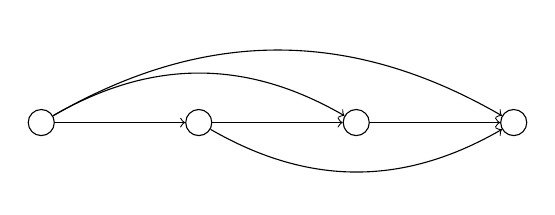
\begin{tikzpicture}
      \node[circle,draw] (1) {};
      \node[circle,draw] (2) [right of=1,xshift=1cm] {};
      \node[circle,draw] (3) [right of=2,xshift=1cm] {};
      \node[circle,draw] (4) [right of=3,xshift=1cm] {};

      \draw[->] (1) -- (2);
      \draw[->] (2) -- (3);
      \draw[->] (3) -- (4);

      \draw[->] (1) edge[bend left] (3);
      \draw[->] (1) edge[bend left] (4);

      \draw[->] (2) edge[bend right] (4);
    \end{tikzpicture}
  \end{center}

  The category \textbf{5} would add one additional object $X$ and 5 additional arrows.
  For every other object $Y$, one arrow would connect $Y$ to $X$; the identity arrow from $X$ to itself is the fifth.

  The category $N$ would consist of an infinite number of objects with one arrow connecting each object to its successor.
  Other arrows follow by composition.

\item[]
\item[1.1.20.4]
  Points (c) and (d) below complete the specification of the category \textbf{M}
  \begin{enumerate}
  \item [(a)]
    the objects of \textbf{M} are the natural numbers;
  \item [(b)]
    an \textbf{M}-arrow $f : m \rightarrow n$ is an $m$-by-$n$ matrix of real numbers;
  \item [(c)]
    the composite $f \circ g$ of two arrows $f : m \rightarrow n$ and $g : n \rightarrow $ is the matrix product of $f$ and $g$.
  \item [(d)]
    the identity arrow of an object $m$ is an $m$-by-$m$ matrix of real numbers
  \item [(e)]
    composition follows by the associativity of matrix multiplication.
  \end{enumerate}

\item[]
\item[1.1.20.5]
  We first present the diagram with generic labels for edges.
  Definitions of the arrow families represented by the labels are given below.

  \begin{center}
    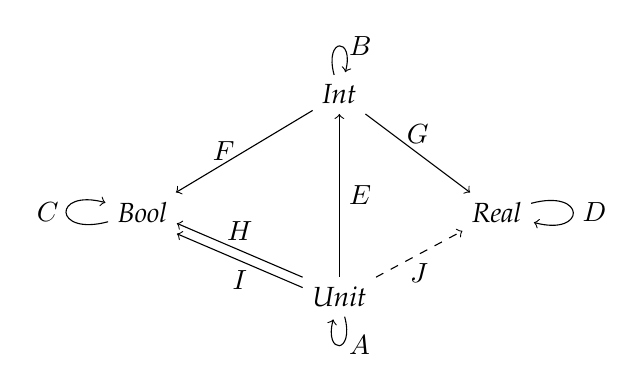
\begin{tikzpicture}
      \node (0) {};
      \node (1) [below of=0,yshift=-2] {\emph{Unit}};
      \node (2) [above of=0,yshift=0.5cm] {\emph{Int}};
      \node (3) [left of=0,xshift=-1.5cm] {\emph{Bool}};
      \node (4) [right of=0,xshift=1cm] {\emph{Real}};

      \draw[->] (1) edge[loop below] node[right] {$A$} (1);
      \draw[->] (1) -- node[right] {$E$} (2);
      \draw[transform canvas={yshift=0.3ex},->] (1) -- node[above] {$H$} (3);
      \draw[transform canvas={yshift=-0.5ex},->] (1) -- node[below] {$I$} (3);
      \draw[dashed,->] (1) -- node[below] {$J$} (4);

      \draw[->] (2) edge[loop above] node[right] {$B$} (2);
      \draw[->] (2) -- node[left] {$F$} (3);
      \draw[->] (2) -- node[above] {$G$} (4);

      \draw[->] (3) edge[loop left] node[right,xshift=-0.5cm] {$C$} (3);

      \draw[->] (4) edge[loop right] node[right] {$D$} (4);

    \end{tikzpicture}
  \end{center}

  \begin{align*}
    A &= (unit~|~id_{unit})*
  \\B &= (succ_{int}~|~id_{int})*
  \\C &= (not~|~id_{bool})*
  \\D &= (succ_{read}~|~id_{real})*
  \\E &= A;~zero;~B
  \\F &= B;~iszero;~C
  \\G &= B;~toreal;~D
  \\H &= A;~true;~C
  \\I &= A;~false;~C
  \\J &= A;~E;~B;~G;~D
  \end{align*}
      
\end{enumerate}
\end{document}
